%%
%% This is file `sigconf-main.tex',
%% generated with the docstrip utility.
%%
%% The original source files were:
%%
%% samples.dtx  (with options: `all,proceedings,bibtex,authordraft')
%% 
%% IMPORTANT NOTICE:
%% 
%% For the copyright see the source file.
%% 
%% Any modified versions of this file must be renamed
%% with new filenames distinct from sample-sigconf-authordraft.tex.
%% 
%% For distribution of the original source see the terms
%% for copying and modification in the file samples.dtx.
%% 
%% This generated file may be distributed as long as the
%% original source files, as listed above, are part of the
%% same distribution. (The sources need not necessarily be
%% in the same archive or directory.)
%%
%%
%% Commands for TeXCount
%TC:macro \cite [option:text,text]
%TC:macro \citep [option:text,text]
%TC:macro \citet [option:text,text]
%TC:envir table 0 1
%TC:envir table* 0 1
%TC:envir tabular [ignore] word
%TC:envir displaymath 0 word
%TC:envir math 0 word
%TC:envir comment 0 0
%%
%% The first command in your LaTeX source must be the \documentclass
%% command.
%%
%% For submission and review of your manuscript please change the
%% command to \documentclass[manuscript, screen, review]{acmart}.
%%
%% When submitting camera ready or to TAPS, please change the command
%% to \documentclass[sigconf]{acmart} or whichever template is required
%% for your publication.
%%
%%
\documentclass[manuscript]{acmart}
%%
%% \BibTeX command to typeset BibTeX logo in the docs
\AtBeginDocument{%
  \providecommand\BibTeX{{%
    Bib\TeX}}}

%% Rights management information.  This information is sent to you
%% when you complete the rights form.  These commands have SAMPLE
%% values in them; it is your responsibility as an author to replace
%% the commands and values with those provided to you when you
%% complete the rights form.
%\setcopyright{""}
%\copyrightyear{""}
%\acmYear{""}
%\acmDOI{""}
%% These commands are for a PROCEEDINGS abstract or paper.
%%\acmConference[]{}
%%
%%  Uncomment \acmBooktitle if the title of the proceedings is different
%%  from ``Proceedings of ...''!
%%
%%\acmBooktitle{Woodstock '18: ACM Symposium on Neural Gaze Detection,
%%  June 03--05, 2018, Woodstock, NY}
%%\acmISBN{}


%%
%% Submission ID.
%% Use this when submitting an article to a sponsored event. You'll
%% receive a unique submission ID from the organizers
%% of the event, and this ID should be used as the parameter to this command.
%%\acmSubmissionID{123-A56-BU3}

%%
%% For managing citations, it is recommended to use bibliography
%% files in BibTeX format.
%%
%% You can then either use BibTeX with the ACM-Reference-Format style,
%% or BibLaTeX with the acmnumeric or acmauthoryear sytles, that include
%% support for advanced citation of software artefact from the
%% biblatex-software package, also separately available on CTAN.
%%
%% Look at the sample-*-biblatex.tex files for templates showcasing
%% the biblatex styles.
%%

%%
%% The majority of ACM publications use numbered citations and
%% references.  The command \citestyle{authoryear} switches to the
%% "author year" style.
%%
%% If you are preparing content for an event
%% sponsored by ACM SIGGRAPH, you must use the "author year" style of
%% citations and references.
%% Uncommenting
%% the next command will enable that style.
%%\citestyle{acmauthoryear}

%% use of package for code snippets
\usepackage{listings}
\usepackage{float}
%% use of package for figures
\usepackage{subcaption}

\lstset{
	language=R,
	basicstyle=\ttfamily\footnotesize,
	backgroundcolor=\color{gray!5},
	frame=single,
	breaklines=true,
	numbers=left,
	numberstyle=\tiny\color{gray},
	keywordstyle=\color{blue},
	commentstyle=\color{gray},
	stringstyle=\color{red!60!black}
}

%%
%% end of the preamble, start of the body of the document source.
\begin{document}

%%
%% The "title" command has an optional parameter,
%% allowing the author to define a "short title" to be used in page headers.
\title{When Scrolling Turns Mindless: A Game-Based Measure of Cognitive Fatigue from Mindless Scrolling}

%%
%% The "author" command and its associated commands are used to define
%% the authors and their affiliations.
%% Of note is the shared affiliation of the first two authors, and the
%% "authornote" and "authornotemark" commands
%% used to denote shared contribution to the research.
\author{Lah Hong Wai}
\affiliation{%
  \institution{Bauhaus-Universität Weimar}
  \city{Weimar}
  \country{Germany}}
\email{lah.hong.wai@uni-weimar.de}

\author{Daniel Radianto}
\affiliation{%
  \institution{Bauhaus-Universität Weimar}
  \city{Weimar}
  \country{Germany}}
\email{daniel.cristianindra.radianto@uni-weimar.de}

\author{Xavier Theodosius}
\affiliation{%
  \institution{Bauhaus-Universität Weimar}
  \city{Weimar}
  \country{Germany}}
\email{xavier.julian.theodosius@uni-weimar.de}

%%
%% By default, the full list of authors will be used in the page
%% headers. Often, this list is too long, and will overlap
%% other information printed in the page headers. This command allows
%% the author to define a more concise list
%% of authors' names for this purpose.
\renewcommand{\shortauthors}{Lah et al.}

%%
%% The abstract is a short summary of the work to be presented in the
%% article.
\begin{abstract}
  With the constant development of smartphones and the ease-of-access to social media, this leads to a constant act of people scrolling through them, as a form of entertainment. This behavior is called mindless-scrolling, which often leads to users losing track of their time easily. Would this behavior also affect their reaction times? To investigate this effect, we designed an experiment with a game that requires participants to select the brighter color. Using a within-subjects design, data were collected from 10 participants who went through one of the two scenarios: calm then mindless-scrolling, and mindless-scrolling then calm. Results show that there were no significant differences between the two conditions, but participants exhibited a slightly faster reaction time for mindless-scrolling.
\end{abstract}

%%
%% The code below is generated by the tool at http://dl.acm.org/ccs.cfm.
%% Please copy and paste the code instead of the example below.
%%
\begin{CCSXML}
<ccs2012>
   <concept>
       <concept_id>10003120.10003121.10011748</concept_id>
       <concept_desc>Human-centered computing~Empirical studies in HCI</concept_desc>
       <concept_significance>500</concept_significance>
       </concept>
   <concept>
       <concept_id>10003120.10003121.10003122.10003334</concept_id>
       <concept_desc>Human-centered computing~User studies</concept_desc>
       <concept_significance>500</concept_significance>
       </concept>
   <concept>
       <concept_id>10010405.10010455.10010459</concept_id>
       <concept_desc>Applied computing~Psychology</concept_desc>
       <concept_significance>300</concept_significance>
       </concept>
 </ccs2012>
\end{CCSXML}

\ccsdesc[500]{Human-centered computing~Empirical studies in HCI}
\ccsdesc[300]{Human-centered computing~User studies}
\ccsdesc[100]{Applied computing~Psychology}

%%
%% Keywords. The author(s) should pick words that accurately describe
%% the work being presented. Separate the keywords with commas.
\keywords{Mindless scrolling, cognitive fatigue, reaction time, experimental game, social media}

%%
%% This command processes the author and affiliation and title
%% information and builds the first part of the formatted document.
\maketitle

\section{Introduction}
Social networks have risen in popularity in the 21st century. They have provided people with a very convenient medium for interaction and sharing. These networks, better known as social media, as defined by Carr and Hayes \cite{Carr2015}, are platforms that enable users to interact and self-present through user-generated content. This emphasizes the communicative and performative dimensions of online interaction, which is imperative to understanding user behaviors such as mindless scrolling.

Multiple studies \cite{deSegovia2024, Ruiz2024, Sinha2023} have been conducted to investigate mindless scrolling on well-being, mental health and focus. One research \cite{Sinha2023} highlighted that typical results are related to a weaker quality of cognitive processing. However, there were no present study that evaluates how mindless-scrolling affects reaction time as a cognitive metric. Therefore, can mindless-scrolling induce a change in reaction time?

\section{Mindless Scrolling and Hypothesis}

The conceptual framework of social media proposed by Carr and Hayes \cite{Carr2015} identifies three core dimensions that explain the prevalence of mindless scrolling: disentrainment (asynchronous communication), persistence (unlimited and continuously accessible content), and perceived interactivity. The interaction among these dimensions encourages even passive users to engage continuously with digital content, often without explicit goals or a defined endpoint. Such engagement creates a behavioral loop that extends screen exposure and progressively diminishes sustained attention.

Building on this foundational understanding of user interaction patterns, Mara Neijzen \cite{Neijzen2024} expands the discussion by introducing the emerging phenomenon of doom behaviour—a broader conceptualization of how individuals engage with information in digital environments. Doom behaviour encompasses doomscrolling, doomsurfing, and doomchecking. Neijzen’s primary objective is to examine whether doom behaviour affects not only prudential outcomes such as anxiety, depression, and sleep deprivation but also epistemic outcomes—whether it enhances or undermines an individual’s understanding of the world. In essence, Neijzen argues that doomscrolling shifts users from goal-directed to stimulus-driven attention, driven by design elements such as endless feeds and persistent notifications. This shift results in short-term lapses of attention, greater exposure to misinformation, and increased cognitive fatigue. Moreover, information overload associated with doomscrolling disrupts the selective attention process and weakens users’ motor responsiveness.

While Neijzen conceptualizes the behavioral and epistemic consequences of doomscrolling, Sinha et al. \cite{Sinha2023} reinforce these claims from a neuropsychological perspective, demonstrating that the infinite-scroll design directly engages the brain’s reward circuitry. Continuous dopaminergic stimulation leads to tolerance, in which users require increasingly intense stimuli to achieve the same level of satisfaction. This neurobiological adaptation contributes to cognitive fatigue, reduces the efficiency of working memory, and slows information-processing speed. Over time, these effects impair the brain’s capacity to sustain prolonged attention and reduce responsiveness to external stimuli, potentially influencing users’ reaction times in everyday activities.

De Segovia Vicente et al. \cite{deSegovia2024} support these findings with empirical evidence derived from experience-sampling methods and behavioral log data. Their study shows that mindless scrolling induces conflicts between users’ intentions and actions (goal conflict), which, in turn, degrade attentional quality and daily cognitive performance. Such degradation is not merely situational but reflects a shift in habitual attention patterns resulting from repeated exposure to high-frequency stimulation embedded in interface design.

Sinha et al. \cite{Sinha2023} further explain that endless scrolling activities create working memory overload and disrupt the brain’s natural segmentation processes for organizing and retaining information. Users exposed to infinite-scroll environments tend to process larger volumes of content but comprehend less, as the absence of structural breaks limits the brain’s ability to consolidate information effectively. Conversely, interface designs incorporating page layouts or stopping cues help users reset focus, enhance spatial orientation, and improve long-term memory encoding. In the context of human performance, such findings imply that limitless interaction designs—such as infinite scroll mechanisms—diminish both the accuracy and speed of responses to subsequent stimuli due to attention fragmentation.
While Sinha et al. \cite{Sinha2023} highlight the neurocognitive mechanisms underlying attentional overload, Hanna \cite{Hanna2022} extends this discussion by explaining how contemporary media environments contribute to cognitive overload. According to Hanna, these effects arise from the endless stream of microtasks co-occurring across social media platforms. Features such as notifications, reels, stories, and continuous feeds divide an individual’s time into microfragments, each demanding brief yet repetitive attention. She attributes this temporal fragmentation to three primary factors: constant notifications and interruptions, algorithmic recommendation systems, and continuous scrolling loops. Collectively, these design features fragment an individual’s attention within minutes, progressively diminishing cognitive capacity and the ability to sustain focus.

Experimental research by Ruiz et al. \cite{Ruiz2024} further advances this discussion through the concept of design friction—small, intentionally introduced interface challenges that serve as cognitive breaks. Within the context of mindless scrolling, friction mechanisms decelerate interaction rhythms and restore users’ situational awareness. Ruiz and colleagues compared two interface prototypes: an infinite-scroll control version and a reaction-based design requiring users to provide feedback before accessing subsequent posts. Their findings reveal that the reaction-based interface enhances content recall, awareness, and cognitive engagement. However, this increase in awareness was accompanied by reduced user satisfaction, suggesting that design interventions must balance attentional regulation with user comfort.

Collectively, these studies demonstrate that mindless scrolling behavior arises from the interplay among user-interface designs that eliminate interaction boundaries, neurobiological responses to rapid gratification, and cognitive mechanisms that reinforce habitual repetition. The consequences extend beyond temporary lapses in focus or memory and may also slow users’ reactions to external stimuli due to adaptation to high-frequency digital stimulation. Within the Human–Computer Interaction (HCI) domain, this body of literature underscores the necessity of interface designs that preserve attentional rhythm, enhance situational awareness, and mitigate compulsive engagement cycles.

Finally, this literature review emphasizes the importance of continued empirical research to examine how mindless scrolling influences reaction time, visual focus, and cognitive endurance in everyday digital interactions. Experimental approaches to measuring cognitive performance would provide critical evidence that bridges the subjective experience of mindless scrolling with objective indicators of human performance in HCI contexts.

Building upon the preceding literature review, the present study aims to empirically investigate how mindless scrolling influences cognitive performance, particularly in the domains of focus and reaction speed. Both theoretical perspectives and empirical findings consistently suggest that infinite scroll designs, algorithmic content delivery, and continuous exposure to online information contribute to declines in attention and increases in cognitive fatigue, which in turn reduce focus and reaction time. Previous studies, such as Sinha et al. \cite{Sinha2023}, further explain that endless scrolling disrupts the brain’s natural segmentation processes and overloads working memory, thereby impairing both attention and reaction efficiency. To further examine how mindless scrolling affects individuals’ attention and response performance, the present study proposes a conceptual framework linking mindless scrolling as the independent variable and reaction time as the dependent variable.
Accordingly, the research hypothesis of this study stated as follows:

\vspace{0.5em}
\noindent\textbf{Hypothesis Statement:} Participants who engage in a set period of mindless scrolling will exhibit significantly slower reaction times on a cognitive task compared to participants who engage in a calming activity.
\vspace{0.5em}

\begin{itemize}
	\item \textbf{H\textsubscript{0}:} There is no significant difference in reaction time between participants who are in an excited state after mindless scrolling and those who are in a relaxed state.
	\item \textbf{H\textsubscript{1}:} Participants who are excited after doing mindless scrolling activity will exhibit significantly slower reaction times compared to those who are in a relaxed state.
\end{itemize}

\section{Method}

\subsection{Participants}

Ten currently enrolled Bauhaus-Universität Weimar students, consisting of five males and five females, with ages that ranged from 22 to 36, volunteered to participate in the study. The participants were active social media users.

\subsection{Experiment Conditions}
The study consisted of two conditions: calm and mindless-scrolling. The calm condition involved the subject listening to relaxation tracks for 10 minutes followed by playing a designated game. The mindless-scrolling condition involved the subject using their smartphone to mindlessly scroll through any of their chosen social media application ten minutes followed by playing the same game as the calm condition. In order to mitigate the carry-over effect, both conditions were separated by a five minute break. The game itself will be explained in the "Dependent Measures" subsection.

\subsection{Materials}

The experiment used several pieces of hardware. The setup that was used by the research subject utilized a MacBook that was connected to a monitor to display the game and the consent form, a speaker for audio playback, and a mouse and keyboard for participant input. The experiment required the subjects to use their own smartphone during the mindless-scrolling conditions of the experiment session. Two researcher smartphones were used for script reading and timing management. Another laptop was also used by the researchers to document the experiment.

\subsection{Dependent Measures}
Following the completion of both the calm and mindless-scrolling condition, a color-picking game is prepared in the subject's experimental setup. The game is relatively simple, it showed two options in forms of boxes with a color of the same hue, but with a luminance gap between the two. Selecting one of the options will finish the round and instantly start another one. The game consisted of 20 consecutive rounds, in which a random color hue was chosen. To increase the task difficulty, the luminance gap between the two options was  decreased by a constant value in as the game progressed. The game is shown in figure~\ref{fig:hci-game}.

\begin{figure}
    \centering
    \includegraphics[width=0.5\linewidth]{figures/hci-game.jpg}
    \caption{Color-picking Game}
    \label{fig:hci-game}
\end{figure}

\subsection{Design}

The study used a within-subjects design and each subject experienced both the calm and the mindless-scrolling conditions. Two sets of sessions were prepared, with each session containing both conditions but in a different order. The sessions in set A started with the calm condition followed by the mindless-scrolling condition. The sessions with set B started with the mindless-scrolling condition followed by the calm condition. The participants were equally and randomly assigned to one of the two sets to counterbalance the order effect. To mitigate the carry-over effects between the two conditions, subjects were given five minute breaks before moving on from the first condition to the second condition. 

\subsection{Procedures}

Subjects were tested individually in the presence of two researchers. One researcher, designated as the "Script Reader", was tasked to introduce the tasks to the subject and let the subject performs the tasks. One researcher, designated as the "Observer", was tasked with documentation of how the experiment was conducted, such as the subject's response to instructions and their expressions throughout the whole session. The observer was also responsible to monitor and verbally signal the completion of the ten minute conditions and the five minute break. 
\par On arrival, the subject was greeted by the script reader and was instructed to sit at a desk, where the experimental setup was prepared (The experimental setup is shown in figure~\ref{fig:study}). The subject was told that they were helping the researchers to measure their reaction time after experiencing two different conditions. The subject was then shown a consent form for them to read. The experiment begun after the subject signed the consent form.








\section{Results}
Participants' reaction times varied across the two conditions. The mean reaction time of participants after mindless-scrolling indicated a slightly faster response time, with better consistency at $sd = 258.68$. The results are shown in Table~\ref{tab:rt_stats}. The descriptive statistics provides an initial overview of the effects of both conditions on cognitive performance.

\begin{table}[ht]
	\caption{Descriptive statistics for reaction time by condition (in ms)}
	\label{tab:rt_stats}
	\centering
	\begin{tabular}{lcc}
		\toprule
		Condition & Mean & SD \\
		\midrule
		Calm & 1214.18 & 370.04 \\
		Mindless & 1133.36 & 258.68 \\
		\bottomrule
	\end{tabular}
\end{table}

\begin{figure}
	\centering
	\includegraphics[width=0.5\linewidth]{figures/descriptive-statistics.png}
	\caption{Reaction times for calm and mindless-scrolling conditions.}
	\label{fig:mean-i-beam}
\end{figure}


A paired sample t-test was performed to identify the effects of mindless-scrolling against a calm condition. The results of the t-test showed no significant difference between the mindless-scrolling and calm scenarios [$t(9) = -1.2014, p = 0.2602$]. 



To further examine on the responsiveness of participants through these conditions, we used Cohen's d to measure the effect size. The result was small to medium, with $d = -0.28$.

\section{Discussion}
The evaluation of the collected data showed that the expected reaction times under the effects of mindless-scrolling were not significant, contrary to the hypothesis. In contrast, participants react faster by $7\%$ from a mean of 1214 $ms$ to 1133 $ms$ after mindless-scrolling than at a calm state. From our observation data, the explanation may be related to our experimental design. Our experimental design consists of a 10 minute calm scenario, which was a rather monotonous session, with participants often shaking legs and fidgeting. Participants have reported that they were extremely bored and therefore began thinking about difficult topics to speed up time. This may have contributed to a slower performance, but results varied more compared to mindless-scrolling ($sd = 370$), implying that performance of participants may be affected by other conditions.

Another possible explanation was that some participants did not unmute their devices while performing the mindless-scrolling task. Playing audio alongside is common when browsing social networks. Although we did not manipulate auditory stimuli, prior research \cite{Chouhan2025, Perez2024} indicate that audio can affect reaction times. Under certain auditory conditions, the reaction times of participants decreased \cite{Perez2024}. Furthermore, the increase in audio loudness directly influences impairment in cognitive performance \cite{Laufs2024}. 

Participants performed the game task with relatively high accuracy in both conditions (mean $>85\%$), which suggests that difference in reaction time were not due to lapses during the tasks. It had also been observed that every participant struggled with the rounds near the end of the game. Therefore, this suggests that there was little flaw with the game design and that it may not have any effect in influencing the results.

\subsection{Limitations}
Due to limited time available when conducting this study, it was acknowledged that the sample size may not be adequate. However, the Cohen's $d = -0.28$ suggests that in a casual setting, there may be little benefit to reaction times between the two conditions.

The caveat of this experiment design has been outlined previously, in that the calm condition was too boring for the participants. Low-stimulus states can lead to increased internal cognitive activity, such as mind-wandering or daydreaming, which can influence reaction times \cite{Deng2022}. Participants may have engaged in these activities over the duration.

Based on the results, even though there was no significant difference, the small-to-medium effect size suggests mindless-scrolling may subtly influence the cognitive readiness. Observation on participants during the calm condition shows that fluctuating cognitive state can be a basis for the reaction time variability.

\subsection{Future Work}
The experiment conducted was small-scale with 10 participants. Future research could explore whether reaction time can be significantly larger with a larger sample size. Demographics and behaviors could also be filtered to provide an insight on the influence. Additionally, it would be valuable to examine if scrolling time and content type would influence results, particularly with negative versus neutral information. Specifically, this would be a comparison between ``doom-scrolling'' against mindless-scrolling.

\section{Conclusion}
This study identified a non-significant result between mindless-scrolling and a calming activity. This contradiction between the result and hypothesis opens questions about whether other conditions could affect reaction times. The results for this study suggests that between the two states, there was not enough evidence to suggest that the mindless-scrolling state will exhibit a significantly slower reaction time on a cognitive task as compared to the other state. It may therefore be advisable to conduct this experiment using a different direction, and avoid any tasks that can be perceived as dull for the participants.
%%
%% The acknowledgments section is defined using the "acks" environment
%% (and NOT an unnumbered section). This ensures the proper
%% identification of the section in the article metadata, and the
%% consistent spelling of the heading.
\begin{acks}
We thank the participants for giving us their time to participate in this experiment. Special recognition goes to Professor Eva and Margarita Osipova for their guidance on this research study. Pramod Bhadana helped with the ideation of this topic. Wang Ruiyu guided with the formatting of this report.
\end{acks}

%%
%% The next two lines define the bibliography style to be used, and
%% the bibliography file.
\bibliographystyle{ACM-Reference-Format}
\bibliography{main-base}


%%
%% If your work has an appendix, this is the place to put it.
\appendix

\section{Use of Large Language Models (LLMs) for Content Development}
This appendix documents the help received from Large Language Models :
\subsection{LLM for Structural Refinement(Gemini)}
\begin{itemize}
    \item \textbf{Tool/Model:} Gemini (Developed by Google)
    \item \textbf{Date of Interaction} 2025-11-08
    \item  \textbf{Purpose:} To refine the structure of the paper and word usage.
    \item \textbf{Prompt Summary:} The prompts focused on the paper's structure, specifically the method section (e.g. In both experiment conditions the subjects will play a color picking game, the condition is explained in a subsection called "Experiments Conditions" where should I explain about the game? Is this explanation repetitive?)
    \item \textbf{Outcome Summary:} The LLM suggested me to explain the game in Materials, Apparatus, or Measures, depending on what the game was used for in the study. The LLM also suggested a few fixes that can be made.
    \item \textbf{Explanation of Use:} I decided to go with the AI's suggestion and put it in the Dependent Measures subsection to show that it was used as a measuring tool. Some words were used too much (e.g. color in the game explanation) and were changed after the interaction concluded.
\end{itemize}

\subsection{LLM for Game Creation (GitHub Copilot)}
\begin{itemize}
    \item \textbf{Tool/Model:} GitHub Copilot
    \item \textbf{Date of Interaction} 2025-11-08
    \item  \textbf{Purpose:} To make the game as a measurement tool for the study.
    \item \textbf{Prompt Summary:} The prompt started with the researcher asking if they should use Client-sided rendering or Server-sided rendering to ensure the fairness of the gameplay between each participant due to the concerns of connection problem caused by the free hosting service. The LLM ended up being used to make and refine the game instead.
    \item \textbf{Outcome Summary:} After the first prompt, the LLM somehow decided to code the whole game. And after further interacting with the researcher, the LLM was used to refine the game until it satisfies the researcher.
    \item \textbf{Explanation of Use:} I had concerns that free hosting may cause connection problem while playing the game, that is what started the first prompt, after the game was automatically coded, I decided to use it to improve the game until it satisfies the whole team.
\end{itemize}

\section{Research Methods}

\subsection{Results of the Experiment}

Table~\ref{tab:appendix_rt} shows data collected from the participants after each condition is done. Data was collected automatically and downloaded into a log file for processing.

\begin{table}[ht]
	\centering
	\caption{Average reaction times (ms) for each participant under Calm and Mindless Scrolling conditions.}
	\label{tab:appendix_rt}
	\begin{tabular}{c c c}
		\toprule
		Participant & Calm (ms) & Mindless Scrolling (ms) \\
		\midrule
		1 & 1615.95 & 1235.45 \\
		2 & 841.25  & 794.55  \\
		3 & 1381.10 & 1081.95 \\
		4 & 1583.90 & 1695.40 \\
		5 & 1580.45 & 1259.35 \\
		6 & 1314.85 & 1148.50 \\
		7 & 579.75  & 780.15  \\
		8 & 721.30  & 770.55  \\
		9 & 1278.05 & 1549.55 \\
		10 & 1352.05 & 1015.65 \\
		\bottomrule
	\end{tabular}
\end{table}

\subsection{Snippet Used for Descriptive Statistics and Analysis}

Statistics were processed with R using TeXStudio. Snippet file can be found at https://nextcloud.uni-weimar.de/s/TRC3MkdLXTFxtWB (pw: ATgqgg4sgQ).

\begin{lstlisting}[caption={Snippet in R}, label={lst:r_code}]
	calm <- c(1615.95, 841.25, 1381.1, 1583.9, 1580.45, 1314.85, 579.75, 721.3, 1278.05, 1352.05)
	mindless <- c(1235.45, 794.55, 1081.95, 1695.4, 1259.35, 1148.5, 780.15, 770.55, 1549.55, 1015.65)
	
	# --- dataframe
	df <- data.frame(
	participant = factor(1:10),
	condition = rep(c("Calm", "Mindless-scrolling"), each = 10),
	rt = c(calm, mindless)
	)
	
	# --- basic statistics
	mean_calm <- mean(calm)
	sd_calm   <- sd(calm)
	mean_mindless <- mean(mindless)
	sd_mindless   <- sd(mindless)
	
	cat("Calm: mean =", round(mean_calm, 2), "sd =", round(sd_calm, 2), "\n")
	cat("Mindless-scrolling: mean =", round(mean_mindless, 2), "sd =", round(sd_mindless, 2), "\n")
	
	# --- paired t test
	tres <- t.test(mindless, calm, paired = TRUE)
	print(tres)
	
	# --- cohen's d
	library(effsize)
	d <- cohen.d(mindless, calm, paired = TRUE)
	print(d)
	
	# --- visualisation
	library(ggplot2)
	library(tidyr)
	
	ggplot(df, aes(x = condition, y = rt)) +
	stat_summary(
	fun = mean, 
	fun.min = function(x) mean(x) - sd(x), 
	fun.max = function(x) mean(x) + sd(x),
	geom = "errorbar", 
	width = 0.1, 
	size = 1
	) +
	stat_summary(fun = mean, geom = "point", size = 4, color = "black") +
	labs(
	x = "Condition",
	y = "Reaction Time (ms)"
	) +
	scale_y_continuous(limits = c(0, 2000)) +
	theme_minimal(base_size = 12)
\end{lstlisting}

\section{Observation Data}

\subsection{Participant Feedback}
Here are the compiled feedback from participants after each session was collected. Only the relevant comments have been listed below.

\begin{itemize}
	\item "The calm session was way too boring. This makes it an unpleasant study for me."
	\item "The entire study was too long."
	\item "It didn't feel like I was actually doom-scrolling. People staring at me made it feel unnatural."
	\item "I usually use social media with sounds. But it was too embarrassing to play it out loud."
	\item "When using the social media, it felt like I was on a train, but instead everyone was judging me. I felt uncomfortable".
\end{itemize}

\subsection{Participant Interaction}

Participants' interaction (who have given consent) are shown below.

\begin{figure}[htbp]
	\centering
	\begin{subfigure}{0.3\textwidth}
		\includegraphics[width=1\linewidth]{figures/p1.jpeg}
	\end{subfigure}
	\begin{subfigure}{0.3\textwidth}
		\includegraphics[width=1\linewidth]{figures/p2.jpeg}
	\end{subfigure}
		\begin{subfigure}{0.3\textwidth}
		\includegraphics[width=1\linewidth]{figures/p3.jpeg}
	\end{subfigure}
	
	\begin{subfigure}{0.3\textwidth}
		\includegraphics[width=1\linewidth]{figures/p4.jpeg}
	\end{subfigure}
		\begin{subfigure}{0.3\textwidth}
		\includegraphics[width=1\linewidth]{figures/p5.jpeg}
	\end{subfigure}
	\begin{subfigure}{0.3\textwidth}
		\includegraphics[width=1\linewidth]{figures/p6.jpeg}
	\end{subfigure}
 \caption{Participants during the interaction.}
	\label{fig:combined-participants}
\end{figure}

\newpage
\section{Study set-up}
This section shows the study set-up that was used for the experiment.
\begin{figure}[htbp]
    \centering
    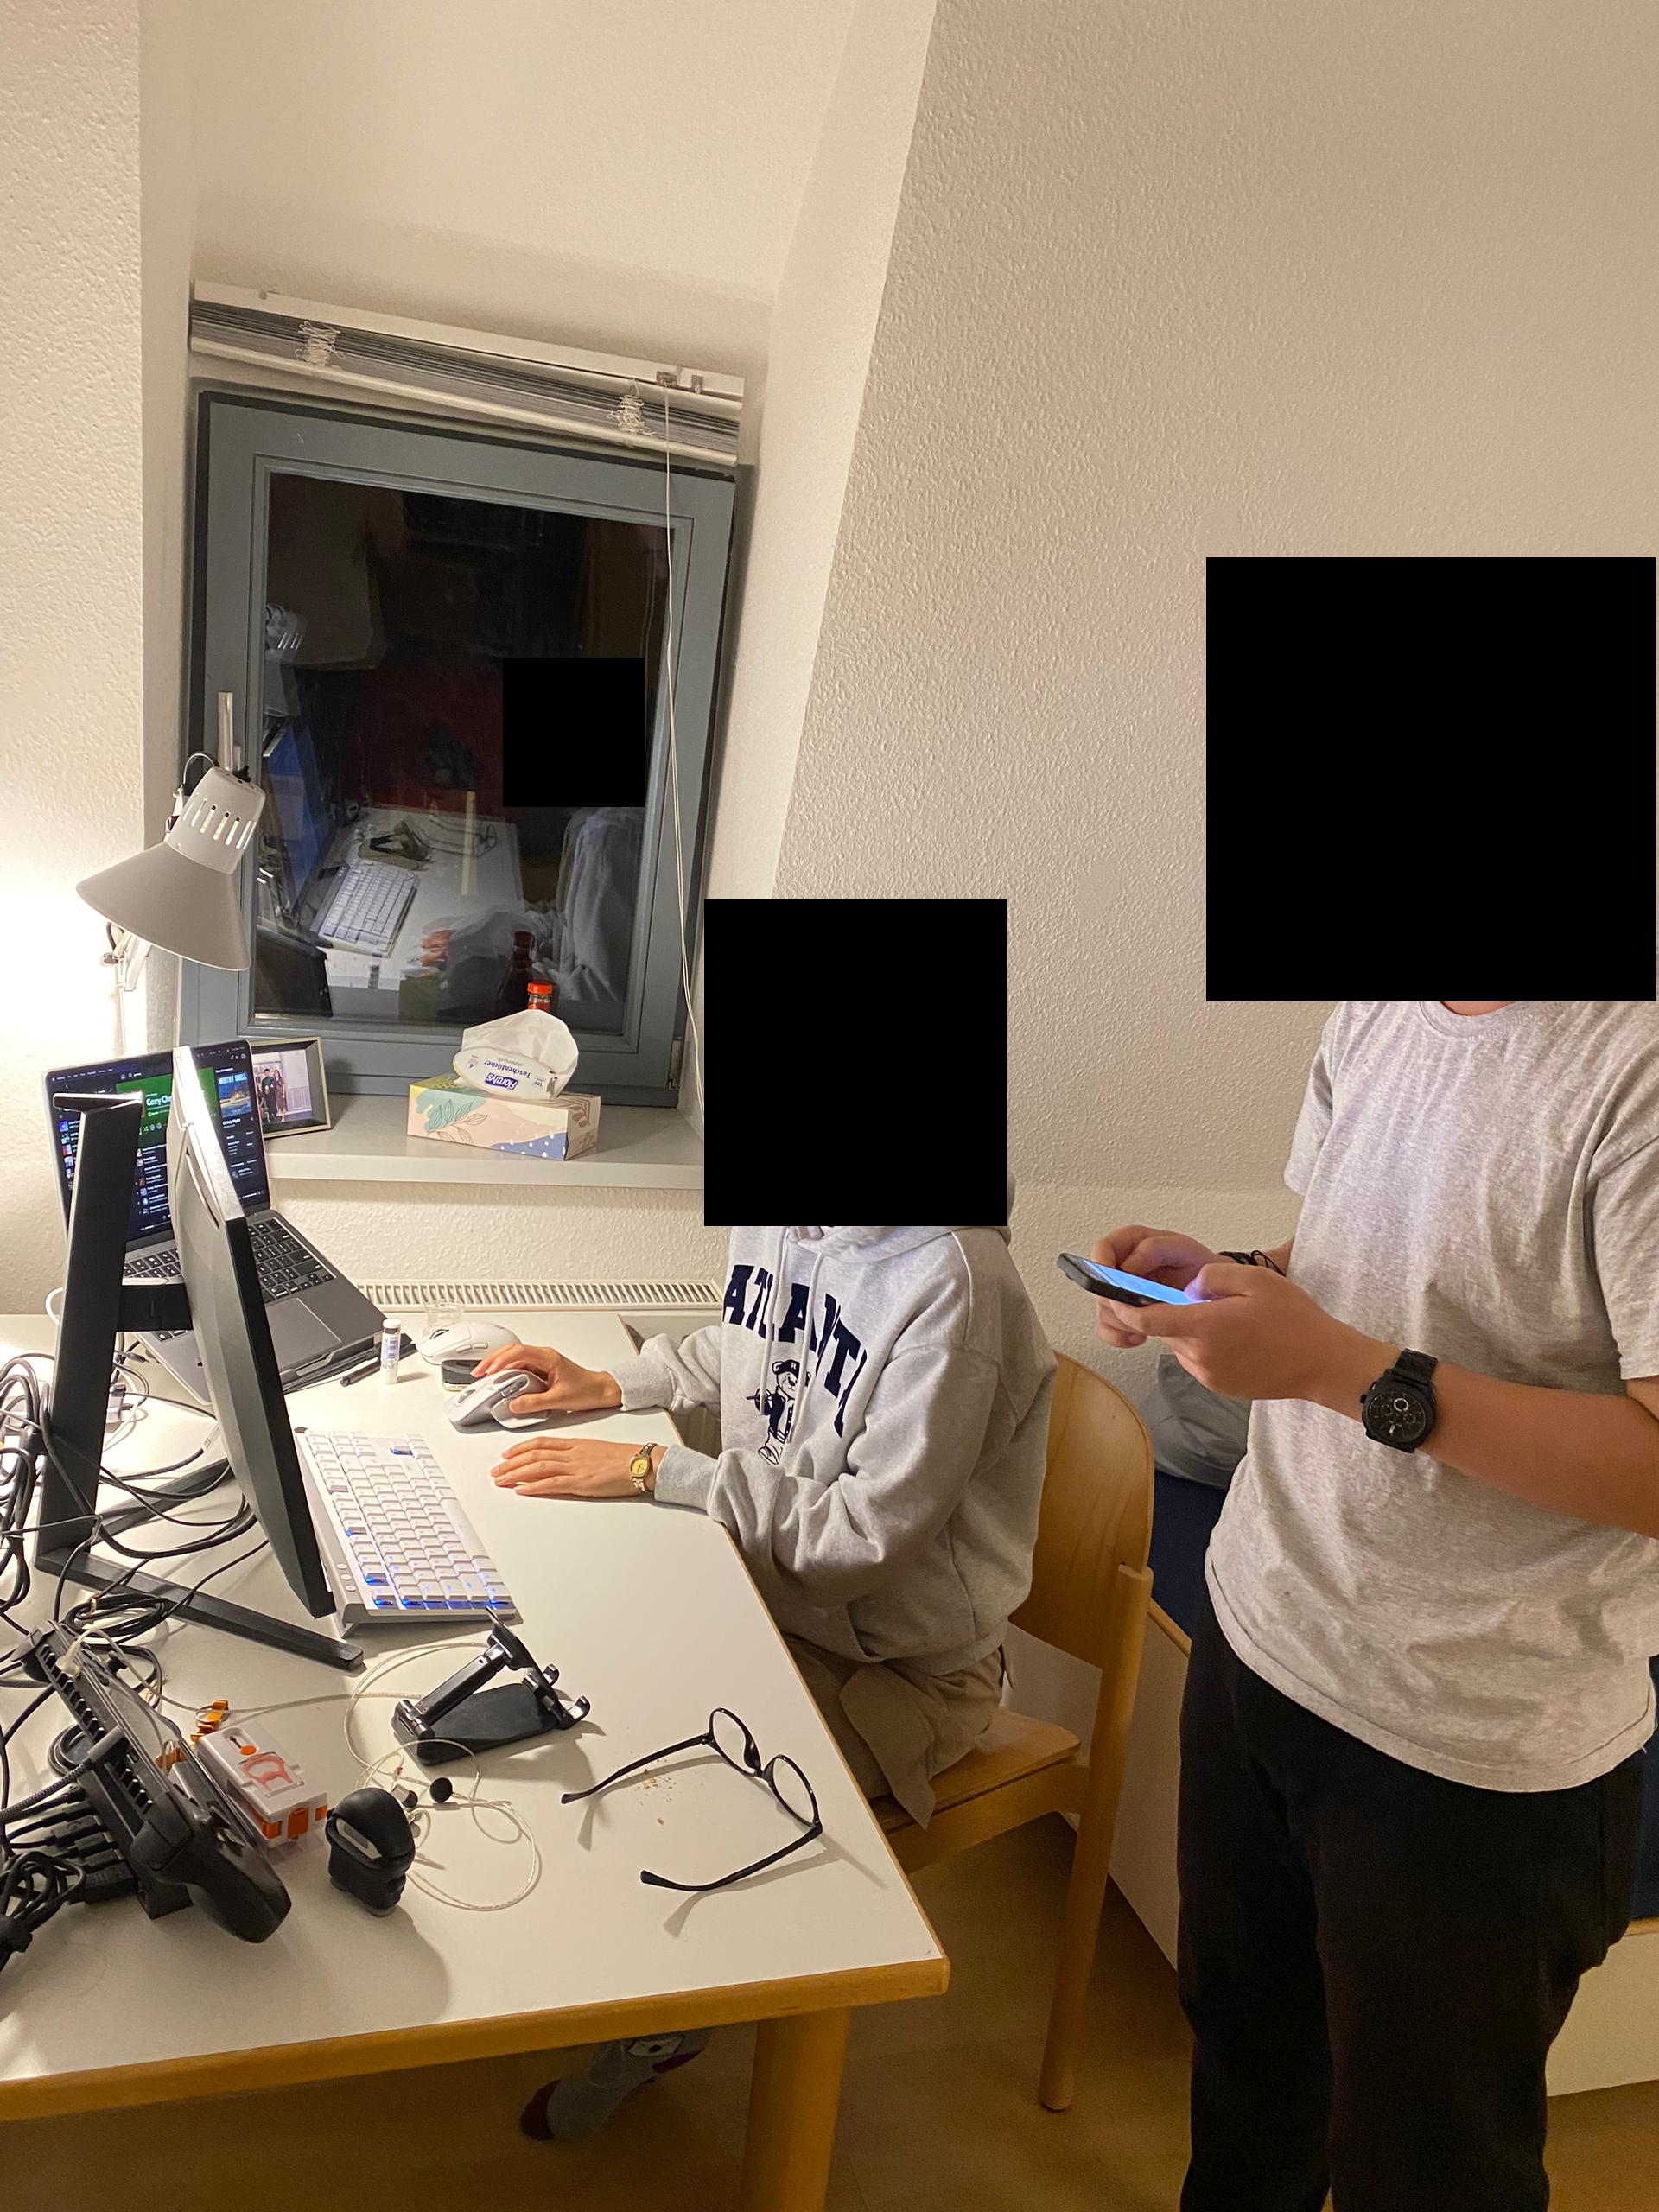
\includegraphics[width=0.5\linewidth]{figures/experiment.png}
    \caption{Study set-up of the experiment}
    \label{fig:study}
\end{figure}



\end{document}
\endinput
%%
%% End of file `sigconf-main.tex'.
